\documentclass[a4paper,12pt]{article}

% \usepackage[latin1]{inputenc}
\usepackage[utf8]{inputenc} 
\usepackage[italian]{babel}
\usepackage{indentfirst}
\usepackage[margin=2.2cm]{geometry}
\usepackage[most]{tcolorbox}
\usepackage{graphicx}
\usepackage{hyperref}
\usepackage[italian]{varioref}
\usepackage{listings}
\usepackage{xcolor}
\usepackage[numbered,framed]{matlab-prettifier}
\usepackage[font={small}]{caption}

\captionsetup[figure]{labelfont={bf},name={Figura},labelsep=period}

\renewcommand{\floatpagefraction}{.8}%
\renewcommand*{\fullref}[1]{\hyperref[{#1}]{\vref*{#1}, \emph{\nameref*{#1}}}}

\graphicspath{{figures/}}


\title{\textbf{Rete Neurale Porta XOR}}
\author{Lara Vignotto}
\date{\today} 


\begin{document}

\maketitle
% \vspace{.5cm}
\vfill
\tableofcontents
\vspace{5cm}


\newpage
%%%%%%%%%%%%%%%%%%%%%%%%%%%%%%
\section{Introduzione e Implementazione}\label{intro}

Vengono qui presentate la progettazione e l'implementazione di una rete neurale che si comporta come una porta logica \texttt{XOR}. È composta da tre strati: un \emph{input layer}, un \emph{hidden layer} e un \emph{output layer} come in Figura \vref{modello}.

\begin{figure}[htb]
    \centering
    \tcbox[boxrule=.3mm,colback=white]{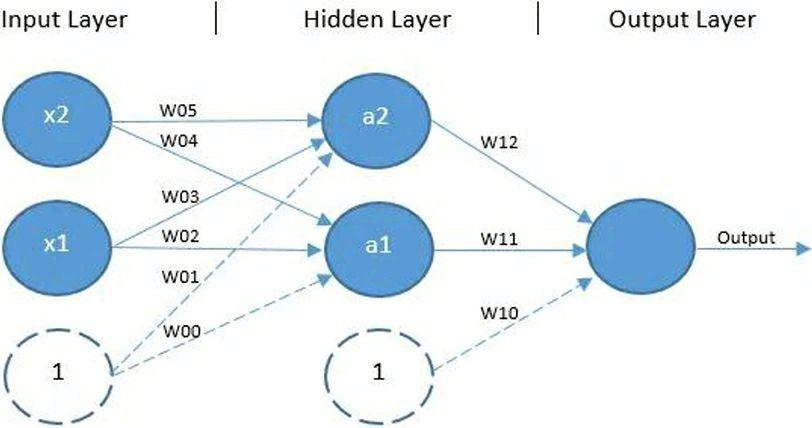
\includegraphics[width=.8\textwidth]{modello.jpg}}
    \caption{Modello di rete neurale: la porta logica XOR.}
    \label{modello}
\end{figure}

Il pacchetto per questa rete neurale è composto da cinque moduli: 2 script e 3 funzioni:

\begin{itemize}
    \item \textbf{Script}:
    \begin{itemize}
        \item \texttt{XOR\_Training}: è stata definita la procedura di apprendimento per la rete neurale. Genera un file con una matrice dei valori dei pesi calcolati a seguito dell'apprendimento;
        \item \texttt{XOR\_Test}: una volta ottenuti i pesi, applica la procedura di apprendimento della rete neurale. Restituisce in output i valori attesi in corrispondenza di ciascun input, in questo caso quattro valori di 0 o 1 a seconda della combinazione di bit data in input.
    \end{itemize}

    \item \textbf{Funzioni}:
    \begin{itemize}
        \item \texttt{XOR\_DeltaRule}: applica la Generalized Delta Rule (GDR). Viene utilizzata ripetutamente nella fase di apprendimento per modificare i valori dei pesi. Questa ripetuta modifica serve a diminuire l'errore, ovvero la differenza tra il valore osservato e quello atteso;
        \item \texttt{Sigmoid};
        \item \texttt{SigmoidDerivative}.
    \end{itemize}
\end{itemize}



\newpage
%%%%%%%%%%%%%%%
\section{Codice}

\begin{lstlisting}[style=Matlab-editor,title=\texttt{XOR\_Training.mat}]
% % Produci un grafico ad ogni run (per grafici punti (4) e (6))
% clear;
% num_run = 5;
% for k = 1:num_run
% figure;
% hold on;
%
alpha = [0.1 0.3 0.5 0.7 0.9];
% alpha = [0.1];
for i = alpha
% %   Prima implementazione
%     vinput = [0 0;
%           0 1;
%           1 0;
%           1 1;
%               ];
%   Seconda implementazione
    vinput = [0 0 1;
            0 1 1;
            1 0 1;
            1 1 1;
                ];
%  
%   I valori attesi in output in corrispondenza di ciascun input  
    correct_output = [0
                    1
                    1
                    0
                    ];

%   Inizializzazione casuale dei pesi
% %   Prima implementazione
%     w0 = 2 * rand(3, 2) - 1;
%     w1 = 2 * rand(1, 3) - 1;
%   Seconda implementazione
    w0 = 2 * rand(3, 3) - 1;
    w1 = 2 * rand(1, 3) - 1;
    w0(3,1) = 0; 
    w0(3,2) = 0; 
    w0(3,3) = 0;
%
% %   Aggiunta di un nodo allo strato nascosto
%     w0 = 2 * rand(4, 3) - 1;
%     w1 = 2 * rand(1, 4) - 1;
%     w0(4,1) = 0; 
%     w0(4,2) = 0; 
%     w0(4,3) = 0;
%
% %   Aggiunta di due nodi allo strato nascosto
%     w0 = 2 * rand(5, 3) - 1;
%     w1 = 2 * rand(1, 5) - 1;
%     w0(5,1) = 0; 
%     w0(5,2) = 0; 
%     w0(5,3) = 0;
%
%   Iperparametro col numero di epoche
    N_epoch = 50000;
%    
%   Inizializzo i vettori per i grafici
    MSE0 = [];          % MSE per epoca
    epoch0 = [];        % epoche
    norm_errors = [];   % norme errori hidden layer
    norm_deltas = [];   % norme delta hidden layer
    i1h1 = [];  % input 1 > hidden 1
    i1h2 = [];  % input 1 > hidden 2
    i1h3 = [];  % input 1 > hidden 3
    i2h1 = [];  % input 2 > hidden 1
    i2h2 = [];  % input 2 > hidden 2
    i2h3 = [];  % input 2 > hidden 3
    h1o = [];   % hidden 1 > output
    h2o = [];   % hidden 2 > output
    h3o = [];   % hidden 3 > output
%
%   Inizia il ciclo di apprendimento sulle epoche
    for epoch = 1:N_epoch
        [w0, w1, final_output, errors_of_hidden_layer, deltas_of_hidden_layer] = XOR_DeltaRule(w0, w1, vinput, correct_output, i);
%
%       Dati per il grafico della curva di apprendimento (loss)
        MSE = immse(final_output, correct_output);  % Mean Squared Error
        MSE0 = [MSE0 MSE];
        epoch0 = [epoch0 epoch];
        norm_errors = [norm_errors norm(errors_of_hidden_layer)];
        norm_deltas = [norm_deltas norm(deltas_of_hidden_layer)];
        %       Dati per le curve dei pesi
        i1h1 = [i1h1 w0(1,1)];
        i1h2 = [i1h2 w0(1,2)];
        i1h3 = [i1h3 w0(2,3)];
        i2h1 = [i2h1 w0(2,1)];
        i2h2 = [i2h2 w0(2,2)];
        i2h3 = [i2h3 w0(2,3)];
        h1o = [h1o w1(1,1)];
        h2o = [h2o w1(1,2)];
        h3o = [h3o w1(1,3)];
%
    end
% %   GRAFICI PUNTO (2)
% %   (2) - 1
% %   Utilizzare alpha = [0.1]; e N_epoch = 50000;
% %   Grafico delle curve di apprendimento con diversi alpha
%     plot(epoch0(1:50000),MSE0(1:50000),'LineWidth',2), grid;
%     title('Learning Curve (Loss)')
%     xlabel('epoch')
%     ylabel('MSE')
%     legend('alpha 0.1', 'alpha 0.3', 'alpha 0.5', 'alpha 0.7', 'alpha 0.9');
%     hold on
%
% %   (2) - 2
% %   Utilizzare alpha = [0.1]; e N_epoch = 50000;
% %   Grafico delle norme dell'errore sullo strato nascosto
%     figure;
%     subplot(1,2,1)
%     plot(epoch0(1:50000),norm_errors(1:50000),'LineWidth',2), grid;
%     title('Norme errore su hidden layer')
%     xlabel('epoch')
%     ylabel('Norma error of hidden layers')
%     legend('alpha 0.1');
%     hold on
% %   Grafico delle norme dei delta dello strato nascosto
%     subplot(1,2,2)
%     plot(epoch0(1:50000),norm_deltas(1:50000),'LineWidth',2), grid;
%     title('Norme delta di hidden layer')
%     xlabel('epoch')
%     ylabel('Norma hidden layer delta')
%     legend('alpha 0.1');
%     hold on
%
% %   GRAFICI PUNTI (4) e (6)
% %   Utilizzare alpha = [0.1, 0.3, ...]; e N_epoch = 10000;
%     plot(epoch0(1:20000),MSE0(1:20000),'LineWidth',2), grid;
%     title('Learning Curve (Loss)')
%     xlabel('epoch')
%     ylabel('MSE')
%     legend('alpha 0.1', 'alpha 0.3', 'alpha 0.5', 'alpha 0.7', 'alpha 0.9');
%
% %   GRAFICI PUNTO (5)
% %   Utilizzare alpha = [0.1]; e N_epoch = 10000;
%     figure('Name','Pesi per alpha = 0.1');
%     
%     subplot(3,3,1);
%     plot(epoch0(1:10000),i1h1(1:10000),'LineWidth',2), grid;
%     title('input 1 > hidden 1')
%     
%     subplot(3,3,2);
%     plot(epoch0(1:10000),i1h2(1:10000),'LineWidth',2), grid;
%     title('input 1 > hidden 2')
%     
%     subplot(3,3,3);
%     plot(epoch0(1:10000),i1h3(1:10000),'LineWidth',2), grid;
%     title('input 1 > hidden 3')
%     
%     subplot(3,3,4);
%     plot(epoch0(1:10000),i2h1(1:10000),'LineWidth',2), grid;
%     title('input 2 > hidden 1')
%     
%     subplot(3,3,5);
%     plot(epoch0(1:10000),i2h2(1:10000),'LineWidth',2), grid;
%     title('input 2 > hidden 2')
%     
%     subplot(3,3,6);
%     plot(epoch0(1:10000),i2h3(1:10000),'LineWidth',2), grid;
%     title('input 2 > hidden 3')
%     
%     subplot(3,3,7);
%     plot(epoch0(1:10000),h1o(1:10000),'LineWidth',2), grid;
%     title('hidden 1 > output')
%     
%     subplot(3,3,8);
%     plot(epoch0(1:10000),h2o(1:10000),'LineWidth',2), grid;
%     title('input 2 > output')
%     
%     subplot(3,3,9);
%     plot(epoch0(1:10000),h3o(1:10000),'LineWidth',2), grid;
%     title('hidden 3 > output')
%
% end
% hold off; % per grafici punti (4) e (6)
end
%
% Memorizzazione su file dei valori dei pesi cosi' calcolati
save('XOR_Trained_Network.mat');
\end{lstlisting}


\newpage
\begin{lstlisting}[style=Matlab-editor,title=\texttt{XOR\_DeltaRule.mat}]
function [w0, w1, final_output, errors_of_hidden_layer, deltas_of_hidden_layer] = XOR_DeltaRule(w0, w1, vinput, correct_output, alpha)
%
%     alpha = 0.9; % Learning rate
    N = size(vinput,1); % Numero di pattern vector nel training set
    final_output = zeros(N,1);
%   Vettori per il grafico della norma dell'errore sullo strato nascosto
    errors = [];
    deltas = [];
    errors_of_hidden_layer = [];
    deltas_of_hidden_layer = [];
%
%   Calcolo sugli input vector (training set)
    for k = 1:N
        transposed_input = vinput(k, :)';
%
%       Fase di feedforward
        input_to_hidden_layer = w0 * transposed_input;
        output_of_hidden_layer = Sigmoid(input_to_hidden_layer);
%
        input_to_output_node = w1 * output_of_hidden_layer;
        final_output(k) = Sigmoid(input_to_output_node);
%       Calcolo dell'errore sullo strato di output
        final_error = correct_output(k) - final_output(k);
        final_delta = final_output(k) * (1 - final_output(k)) * final_error;
%
%       Fase di backpropagation
        error_of_hidden_layer = w1' * final_delta;
        hidden_layer_delta = SigmoidDerivative(output_of_hidden_layer) .* error_of_hidden_layer;
%       Dati per il grafico della norma dell'errore sullo strato nascosto
        errors = [errors error_of_hidden_layer(1:2)];
        deltas = [deltas hidden_layer_delta(1:2)];
%
%       Calcolo delle correzioni da applicare ai pesi
        dW1 = alpha * final_delta * output_of_hidden_layer';
        dW0 = alpha * hidden_layer_delta * transposed_input';
%       Applicazione delle correzioni (Generalized Delta Rule)
        w0 = w0 + dW0;
        w1 = w1 + dW1;
%       Azzeramento dei pesi ridondanti
        w0(3,1) = 0; 
        w0(3,2) = 0; 
        w0(3,3) = 0;
% %         aggiunta di 1 nodo nascosto
%         w0(4,1) = 0; 
%         w0(4,2) = 0; 
%         w0(4,3) = 0;
% %         aggiunta di 2 nodi nascosti
%         w0(5,1) = 0; 
%         w0(5,2) = 0; 
%         w0(5,3) = 0;
    end 
%   Dati per il grafico della norma dell'errore sullo strato nascosto
    errors_of_hidden_layer = [errors_of_hidden_layer errors];
    deltas_of_hidden_layer = [deltas_of_hidden_layer deltas];
end
\end{lstlisting}

\vspace{1cm}

% \newpage
\begin{lstlisting}[style=Matlab-editor,title=\texttt{Sigmoid.mat}]
function y = Sigmoid(x)
    y = 1./(1+exp(-x));
end
\end{lstlisting}

\vspace{1cm}

\begin{lstlisting}[style=Matlab-editor,title=\texttt{SigmoidDerivative.mat}]
function y = SigmoidDerivative(x)
    if (isscalar(x))
        y = x * (1-x);
    else
        y = x .* (1-x);
    end
end
\end{lstlisting}

\vspace{1cm}

\begin{lstlisting}[style=Matlab-editor,title=\texttt{XOR\_Test.mat}]
% Carica i dati della rete gia' addestrata
load('XOR_Trained_Network.mat')
%
transposed_input = vinput(1, :)';
input_to_hidden_layer = w0 * transposed_input;
output_of_hidden_layer = Sigmoid(input_to_hidden_layer);
%
input_to_output_node = w1 * output_of_hidden_layer;
final_output(1) = Sigmoid(input_to_output_node)
\end{lstlisting}



\newpage
%%%%%%%%%%%%%%%%%%%%%%%%%%%%%%
\section{Osservazioni e Conclusioni}

Abbiamo attuato diverse verifiche e analisi per implementare e scegliere il modello di rete neurale più efficiente.


\setcounter{subsection}{-1}
%%%%%%%%%%%%%%%%
\subsection{Confronto fra due implementazioni}

Abbiamo provato due diverse implementazioni e le abbiamo confrontate per stabilire quale delle due fosse la più efficiente.

\subsubsection{Prima implementazione}
Il peso \texttt{w0} è stato definito come una matrice $3\times 2$, mentre \texttt{vinput} è $4\times 2$. Abbiamo tracciato la curva di apprendimento loss per cinque diversi valori di $\alpha$ (Figura~\vref{fig0-first-implementation}).

\begin{figure}[htb]
    \centering
    \tcbox[boxrule=.3mm,colback=white]{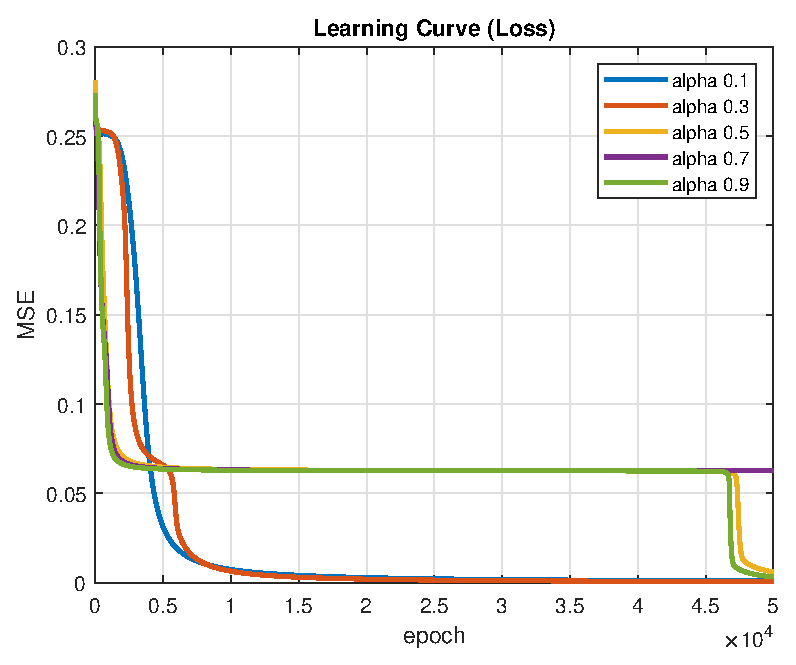
\includegraphics[width=.9\textwidth]{fig0-first-implementation.eps}}
    \caption{Prima implementazione: curve di apprendimento al variare di $\alpha$.}
    \label{fig0-first-implementation}
\end{figure}

\subsubsection{Seconda implementazione}
Abbiamo aggiunto il nodo bias al primo strato, come se l'input fosse a 3 bit. Il peso \texttt{w0} è quindi ora una matrice $3\times 3$, mentre \texttt{vinput} è $4\times 3$. Lo schema vuole 6 pesi, ma noi ne abbiamo definiti 9 aggiungendo un terzo nodo nello strato nascosto. Per ``controllare'' questa ridondanza abbiamo settato a 0 i pesi \texttt{w0(3,1)}, \texttt{w0(3,2)} e \texttt{w0(3,3)} sia in \texttt{XOR\_Training} che in \texttt{XOR\_DeltaRule}. In Figura~\vref{fig0-second-implementation} si può osservare la curva di apprendimento loss per cinque diversi valori di $\alpha$.

\begin{figure}[htb]
    \centering
    \tcbox[boxrule=.3mm,colback=white]{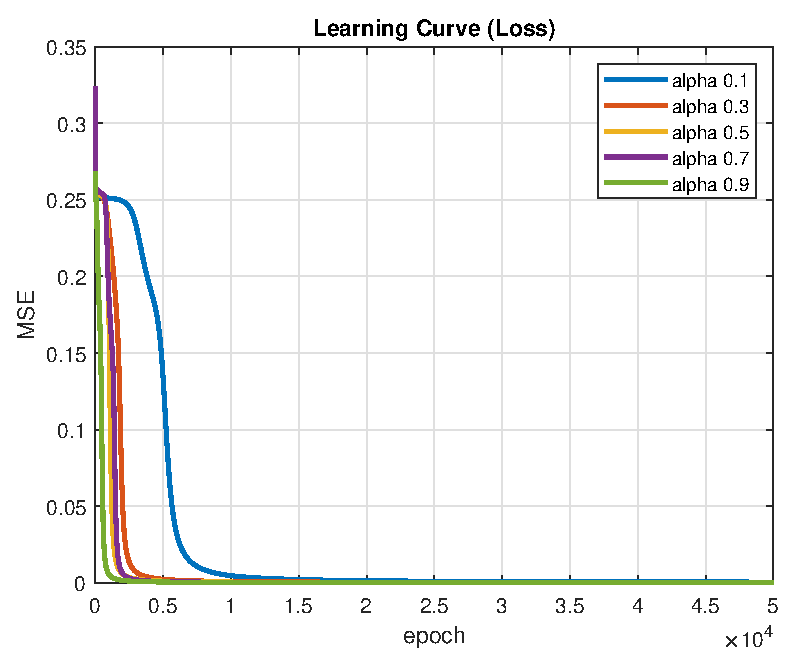
\includegraphics[width=.9\textwidth]{fig0-second-implementation.eps}}
    \caption{Seconda implementazione: curve di apprendimento al variare di $\alpha$.}
    \label{fig0-second-implementation}
\end{figure}

\subsubsection{Osservazioni}

Si osserva che nella prima implementazione alcune curve faticano a convergere, o non lo fanno proprio (Figura~\vref{fig0-first-implementation}), mentre con la seconda implementazione tutte le curve convergono sempre.

Per spiegare questo fenomeno si può fare un'ipotesi. Il comportamento delle curve nella prima implementazione potrebbe essere dovuto all'effetto di \textbf{saturazione}. La funzione di attivazione, infatti, dovrebbe essere una sigmoide, quindi variare tra 0 e 1. Se, per effetti numerici, si sposta troppo vicino a 0 o troppo vicino a 1, ovvero agli estremi, tende a rimanere ``intrappolata''. Di conseguenza non converge, restituisce un output (MSE) sempre uguale.

Visti questi risultati, decidiamo di procedere con la seconda implementazione, in quanto appare come più efficiente.



%%%%%%%%%%%%%%%%
\subsection{Progettazione e implementazione}
Si veda la sezione~\fullref{intro}.



\newpage
%%%%%%%%%%%%%%%%
\subsection{Prima verifica dell'apprendimento: analisi dell'errore}\label{prima-verifica}
Abbiamo già calcolato le curve loss per cinque valori del parametro alpha ($0.1$, $0.3$, $0.5$, $0.7$ e $0.9$). Il grafico risultante è in Figura~\vref{fig0-second-implementation}. Osserviamo come in 50000 epoche le curve convergono sempre. Considerazioni più significative vengono fatte al punto \fullref{analisi-stabilita}.\medskip

Abbiamo calcolato in seguito il diagramma con alpha $= 0.1$ della norma dell’errore sullo strato nascosto rispetto alle epoche (Figura~\vref{fig2-2}).  

\begin{figure}[htb]
    \centering
    \tcbox[boxrule=.3mm,colback=white]{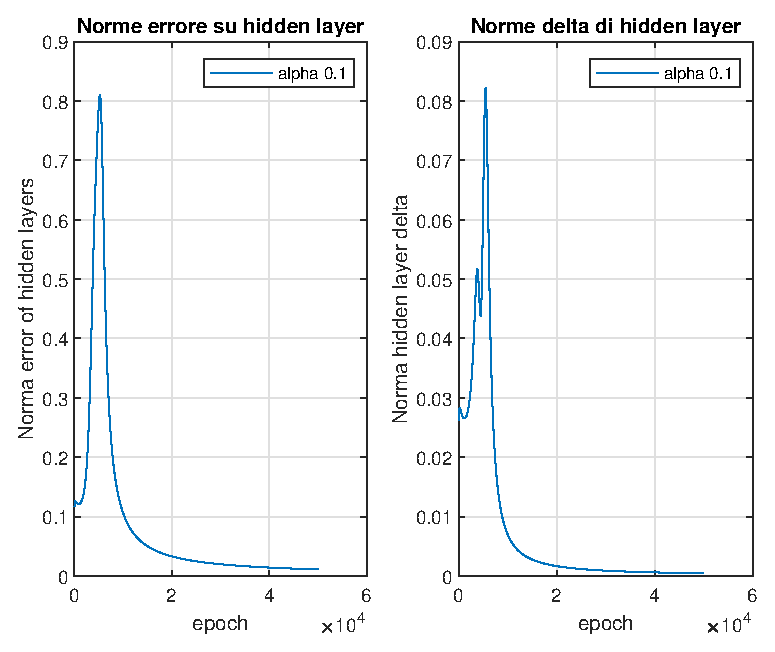
\includegraphics[width=.9\textwidth]{fig2-2.eps}}
    \caption{Norma dell’errore sullo strato nascosto rispetto alle epoche. Sull'asse $y$, a sinistra è stata calcolata la norma su \texttt{error\_of\_hidden\_layers}, a destra è stata calcolata la norma su \texttt{hidden\_layer\_delta}.}
    \label{fig2-2}
\end{figure}

Si può osservare che c'è una differenza di scala tra i due grafici: la norma dell'errore sullo strato nascosto (grafico a sinistra) è di un'ordine di grandezza maggiore alla norma dell'errore sul delta (grafico a destra).



\newpage
%%%%%%%%%%%%%%%%
\subsection{Seconda verifica dell'apprendimento: configurazione della rete}

Abbiamo visualizzato la configurazione del modello istanziato dopo l’apprendimento, ovvero il file \texttt{XOR\_Trained\_Network.mat}:

\begin{lstlisting}[style=Matlab-editor]
matjob = 

  matlab.io.MatFile

  Properties:
         Properties.Source: 'E:\Users\...\XOR_Trained_Network.mat'
       Properties.Writable: false                                                                 
                       MSE: [1x1     double]                                                      
                      MSE0: [1x50000 double]                                                      
                   N_epoch: [1x1     double]                                                      
                     alpha: [1x1     double]                                                      
            correct_output: [4x1     double]                                                      
    deltas_of_hidden_layer: [2x4     double]                                                      
                     epoch: [1x1     double]                                                      
                    epoch0: [1x50000 double]                                                      
    errors_of_hidden_layer: [2x4     double]                                                      
              final_output: [4x1     double]                                                      
                         i: [1x1     double]                                                      
               norm_deltas: [1x50000 double]                                                      
               norm_errors: [1x50000 double]                                                      
                    vinput: [4x3     double]                                                      
                        w0: [3x3     double]                                                      
                        w1: [1x3     double] 
\end{lstlisting}

Questa verifica è stata eseguita usando la procedura \texttt{matfile()}, che ha permesso di osservare la memoria di lavoro dopo che è avvenuto l'apprendimento. \texttt{XOR\_Trained\_Network.mat} contiene attributi e valori che registrano i parametri dell'apprendimento.



\newpage
%%%%%%%%%%%%%%%%
\subsection{Analisi di stabilità}\label{analisi-stabilita}

Abbiamo ripetuto il calcolo eseguito al punto \fullref{prima-verifica} per cinque volte. Il risultato sono stati cinque grafici di curve di apprendimento loss su 20000 epoche (Figure~\vref{fig4}, \vref{fig4-2} e \vref{fig4-3}).

Osserviamo che in alcuni casi la curva converge sempre, in particolare con alpha $= 0.1$. Al contrario, per alcuni valori di alpha la curva presenta delle instabilità: in particolare nel primo e secondo grafico la curva verde ($\alpha=0.9$) e nel terzo grafico quella gialla ($\alpha=0.5$) non convergono.

Uteriori osservazioni sono state fatte al punto \fullref{analisi-efficacia} con il confronto con altri modelli di rete neurale.

\begin{figure}[htb]
    \centering
    \tcbox[boxrule=.3mm,colback=white]{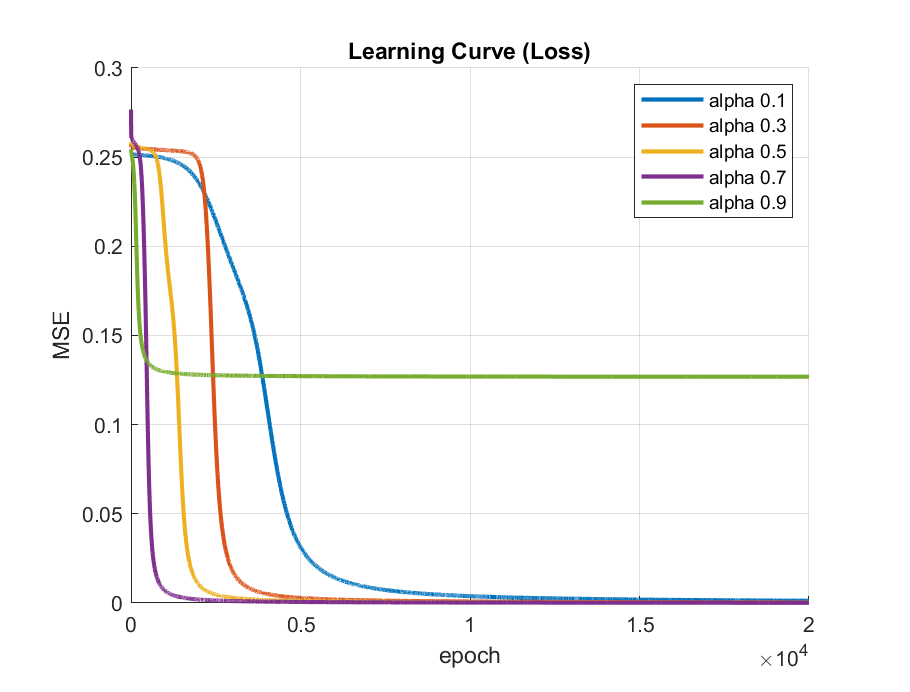
\includegraphics[width=.9\textwidth]{fig4-1.eps}}
    \caption{Curve di apprendimento loss (1/5): seconda implementazione, 2 nodi nello strato nascosto.}
    \label{fig4}
\end{figure}

\begin{figure}[htp]
    \centering
    \tcbox[boxrule=.3mm,colback=white]{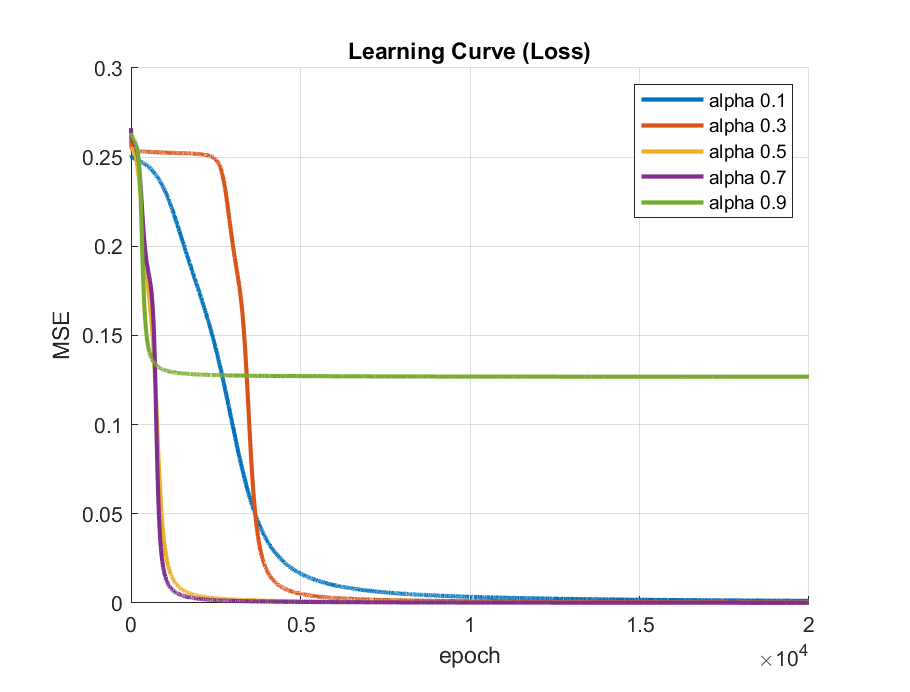
\includegraphics[width=.9\textwidth]{fig4-2.eps}}

    \medskip

    \tcbox[boxrule=.3mm,colback=white]{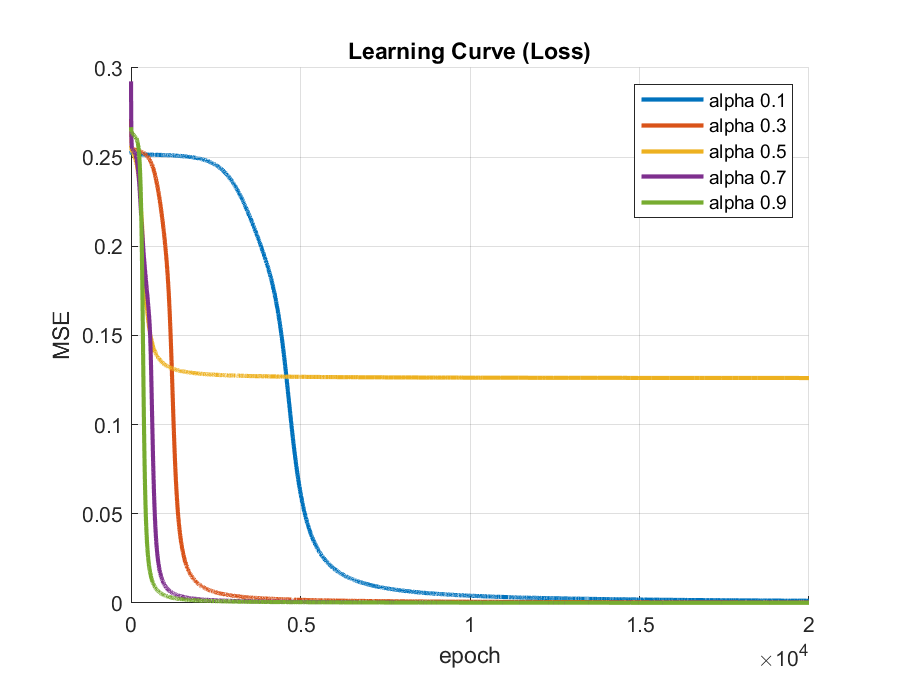
\includegraphics[width=.9\textwidth]{fig4-3.eps}}

    \caption{Curve di apprendimento loss (2/5 e 3/5): seconda implementazione, 2 nodi nello strato nascosto.}
    \label{fig4-2}
\end{figure}

\begin{figure}[htp]
    \centering
    \tcbox[boxrule=.3mm,colback=white]{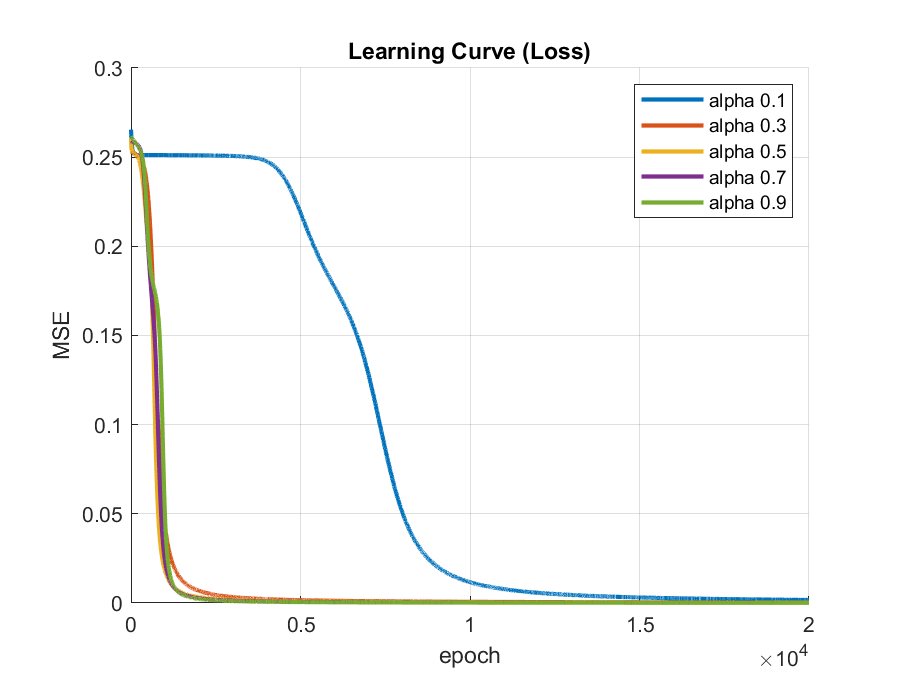
\includegraphics[width=.9\textwidth]{fig4-4.eps}}

    \medskip

    \tcbox[boxrule=.3mm,colback=white]{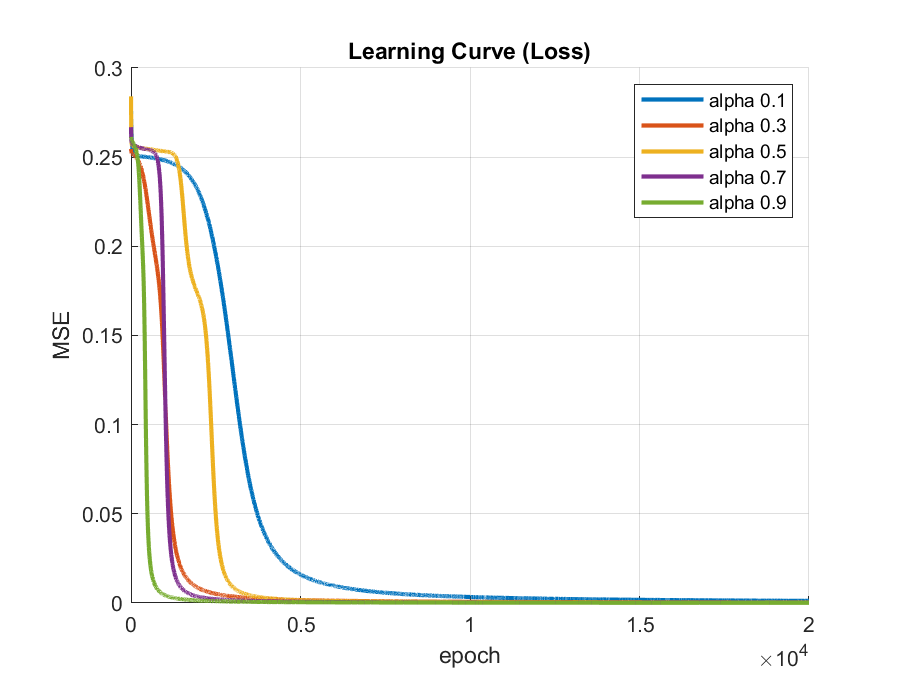
\includegraphics[width=.9\textwidth]{fig4-5.eps}}

    \caption{Curve di apprendimento loss (4/5 e 5/5): seconda implementazione, 2 nodi nello strato nascosto.}
    \label{fig4-3}
\end{figure}



\newpage
%%%%%%%%%%%%%%%%
\subsection{Terza verifica dell'apprendimento: analisi dei pesi}

Al punto \fullref{prima-verifica} abbiamo valutato come miglior alpha il valore $0.1$. Fissando $\alpha = 0.1$ abbiamo calcolato l'andamento di cascuno dei pesi $w_{ij}$ durante l'apprendimento. I nove grafici singoli sono riportati in Figura~\vref{fig5}.

\begin{figure}[htb]
    \centering
    \tcbox[boxrule=.3mm,colback=white]{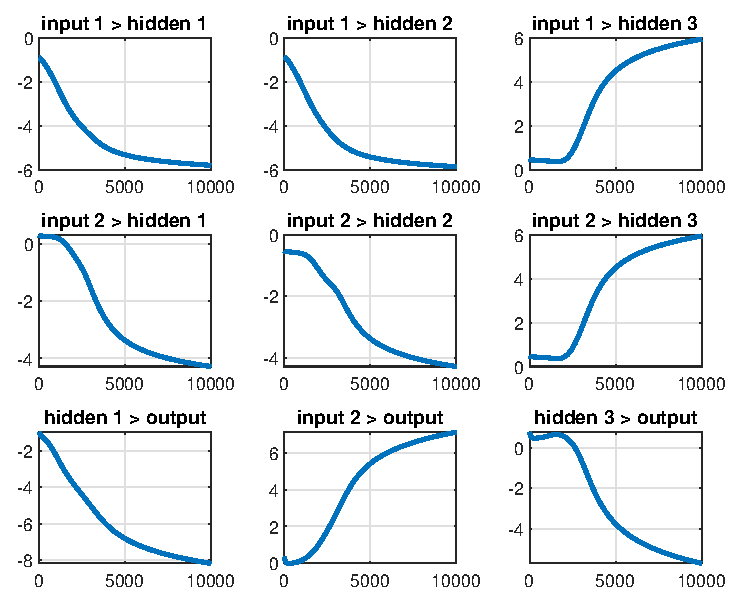
\includegraphics[width=.9\textwidth]{fig5-2.eps}}
    \caption{Variare dei valori dei pesi in funzione delle epoche per ognuno dei nove pesi.}
    \label{fig5}
\end{figure}



\newpage
%%%%%%%%%%%%%%%%
\subsection{Analisi di efficacia del modello}\label{analisi-efficacia}

Abbiamo aggiunto un nodo nascosto al modello e abbiamo ripetuto il calcolo effettuato al punto \fullref{analisi-stabilita}. I cinque grafici risultanti sono riportati nelle Figure~\vref{fig6},~\vref{fig6-2} e~\vref{fig6-3}.

\begin{figure}[htb]
    \centering
    \tcbox[boxrule=.3mm,colback=white]{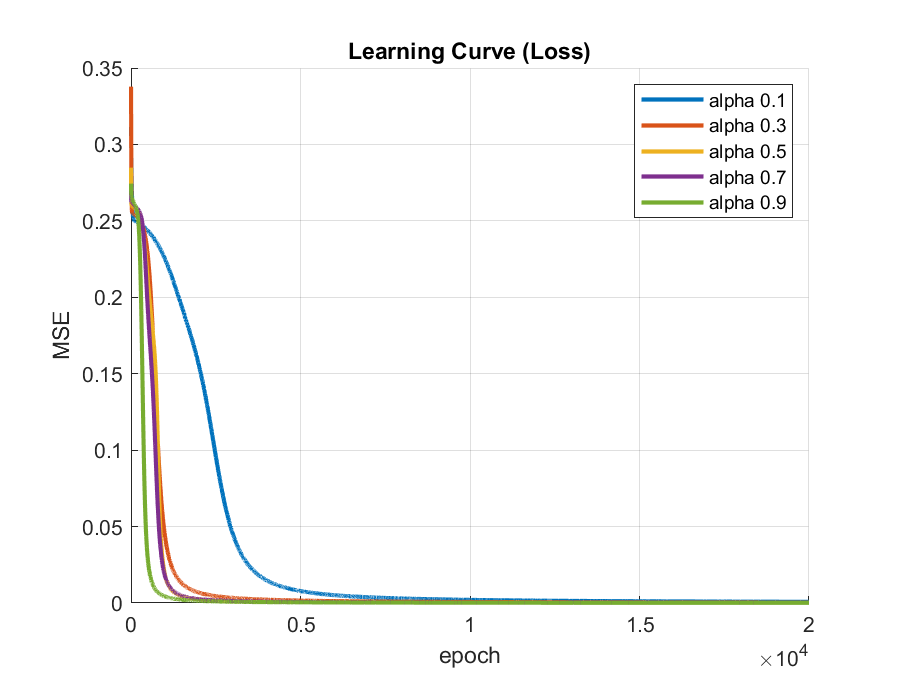
\includegraphics[width=.9\textwidth]{fig6-3nodi-1.eps}}
    \caption{Curve di apprendimento loss (1/5): seconda implementazione, 3 nodi nello strato nascosto.}
    \label{fig6}
\end{figure}

\begin{figure}[htp]
    \centering
    \tcbox[boxrule=.3mm,colback=white]{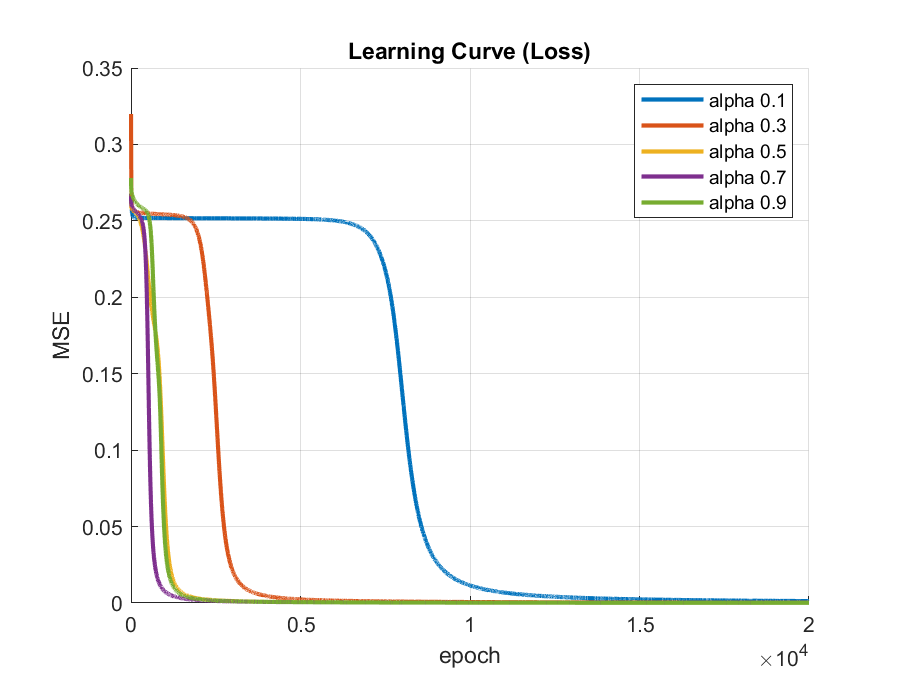
\includegraphics[width=.9\textwidth]{fig6-3nodi-2.eps}}

    \medskip

    \tcbox[boxrule=.3mm,colback=white]{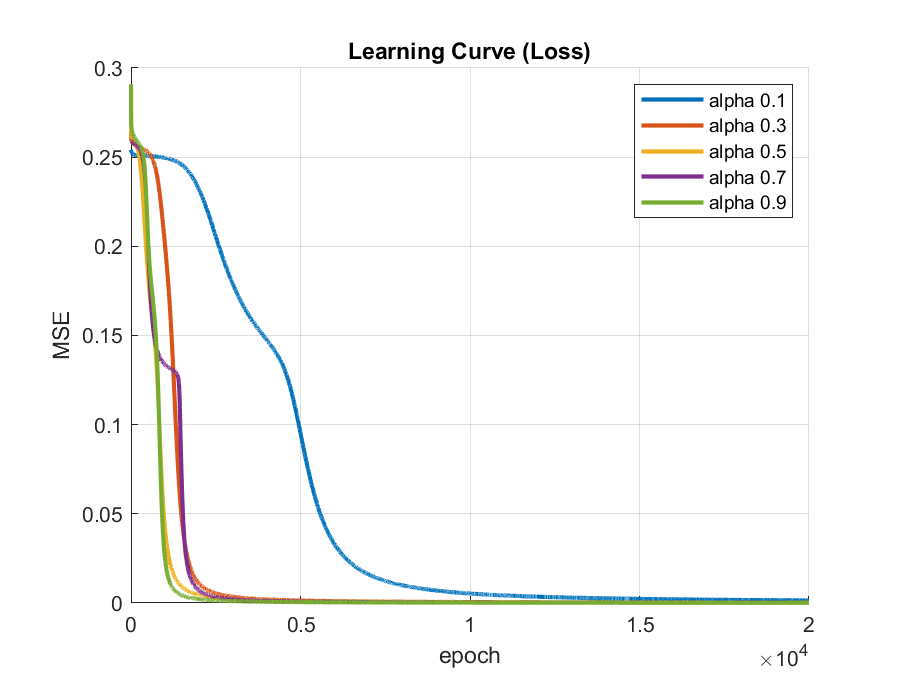
\includegraphics[width=.9\textwidth]{fig6-3nodi-3.eps}}

    \caption{Curve di apprendimento loss (2/5 e 3/5): seconda implementazione, 3 nodi nello strato nascosto.}
    \label{fig6-2}
\end{figure}

\begin{figure}[htp]
    \centering
    \tcbox[boxrule=.3mm,colback=white]{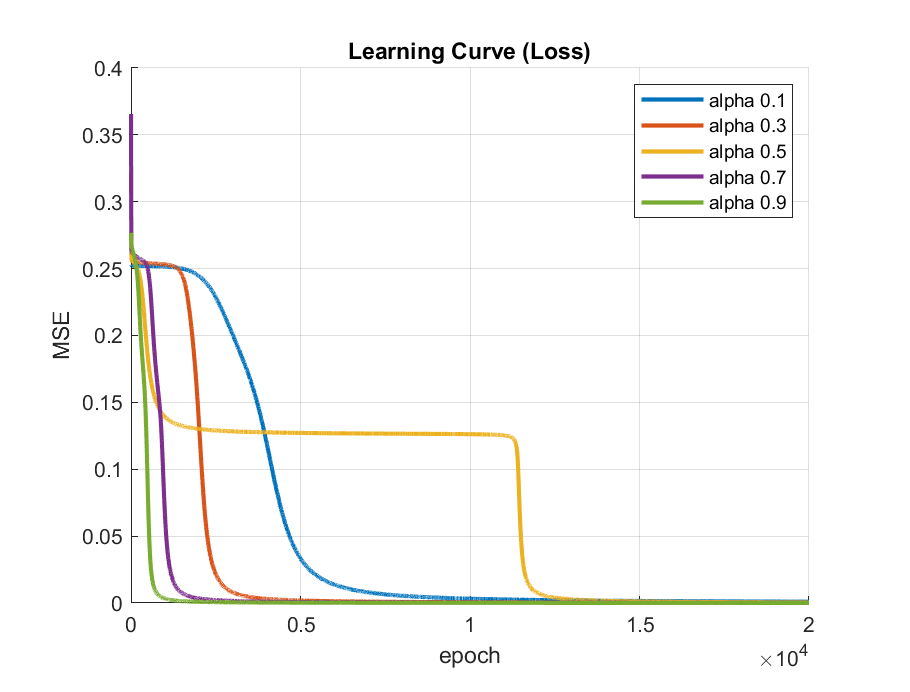
\includegraphics[width=.9\textwidth]{fig6-3nodi-4.eps}}

    \medskip

    \tcbox[boxrule=.3mm,colback=white]{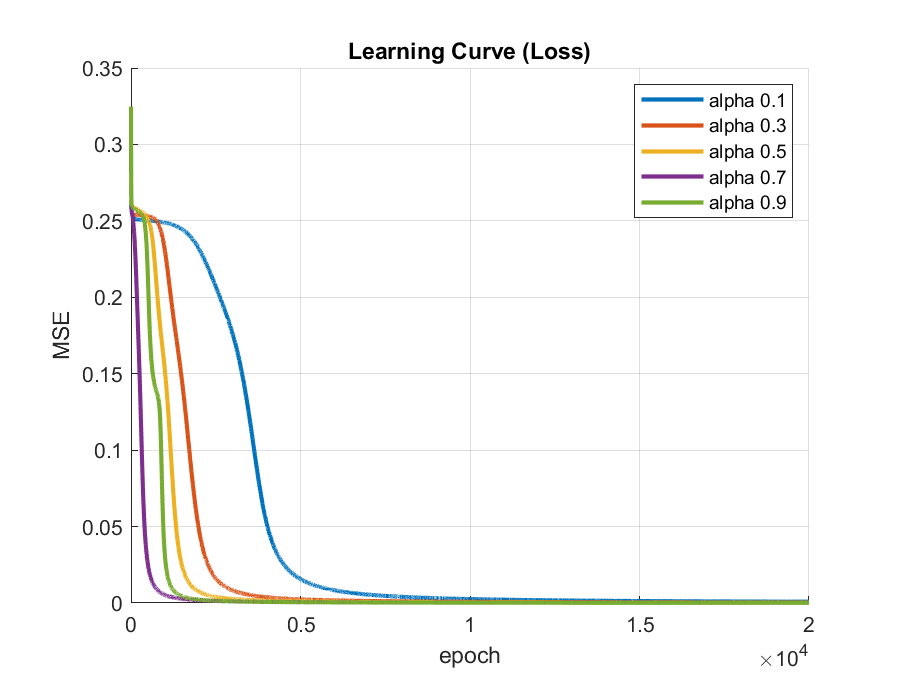
\includegraphics[width=.9\textwidth]{fig6-3nodi-5.eps}}

    \caption{Curve di apprendimento loss (4/5 e 5/5): seconda implementazione, 3 nodi nello strato nascosto.}
    \label{fig6-3}
\end{figure}



\newpage
Lo stesso calcolo è stato fatto aggiungendo due nodi nascosti, e il risultato si può osservare nelle Figure~\vref{fig6-4},~\vref{fig6-5} e~\vref{fig6-6}.

\begin{figure}[htb]
    \centering
    \tcbox[boxrule=.3mm,colback=white]{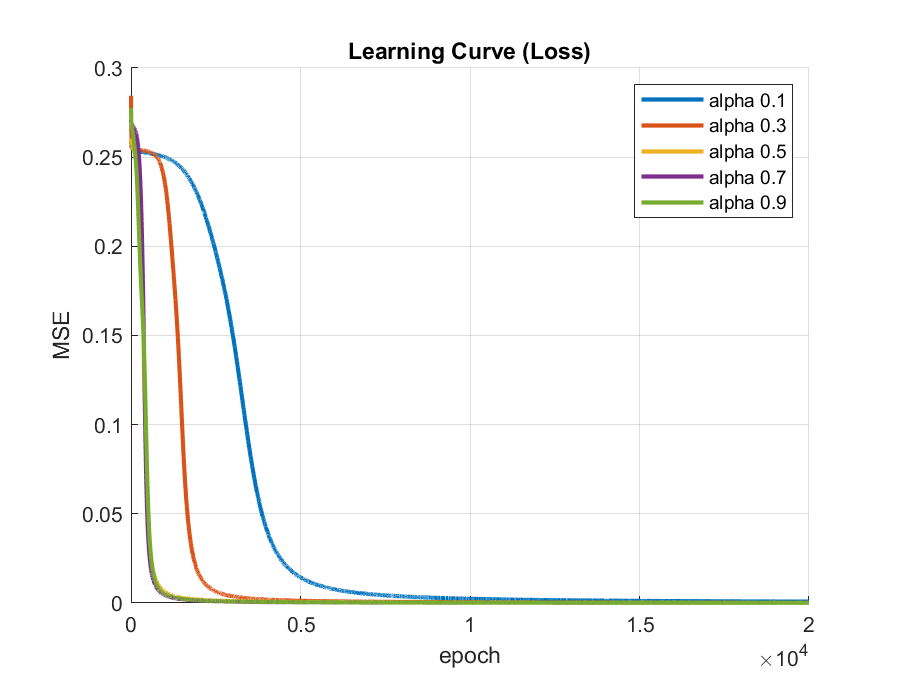
\includegraphics[width=.9\textwidth]{fig6-4nodi-1.eps}}
    \caption{Curve di apprendimento loss (1/5): seconda implementazione, 4 nodi nello strato nascosto.}
    \label{fig6-4}
\end{figure}

\begin{figure}[htp]
    \centering
    \tcbox[boxrule=.3mm,colback=white]{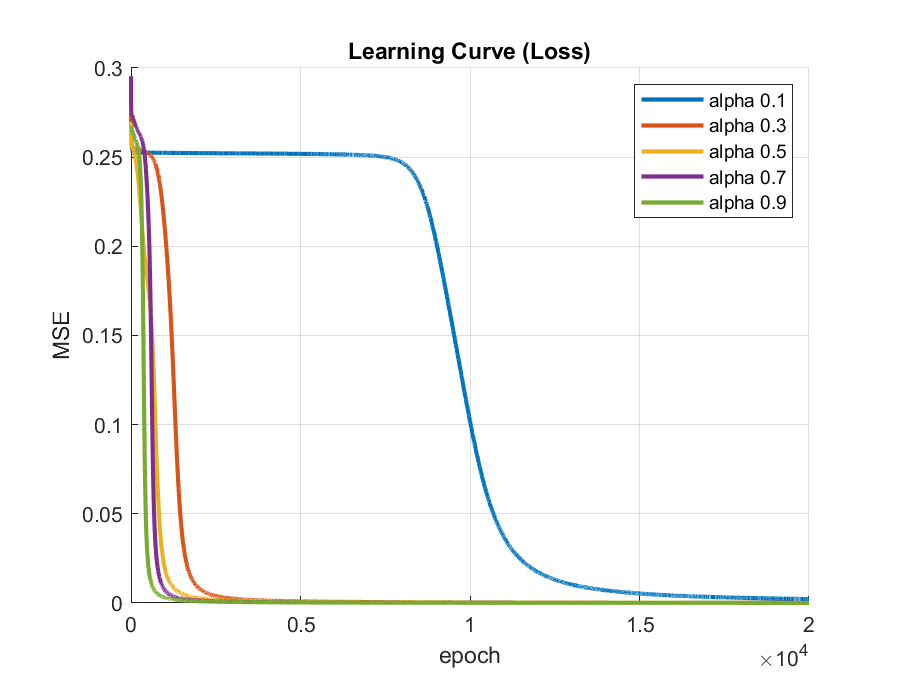
\includegraphics[width=.9\textwidth]{fig6-4nodi-2.eps}}

    \medskip

    \tcbox[boxrule=.3mm,colback=white]{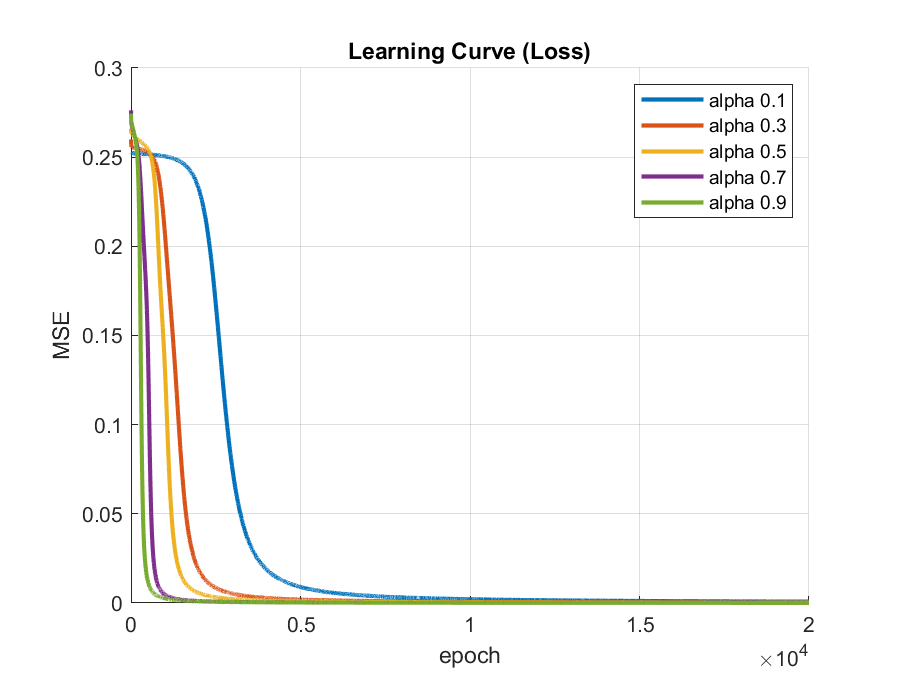
\includegraphics[width=.9\textwidth]{fig6-4nodi-3.eps}}

    \caption{Curve di apprendimento loss (2/5 e 3/5): seconda implementazione, 4 nodi nello strato nascosto.}
    \label{fig6-5}
\end{figure}

\begin{figure}[htp]
    \centering
    \tcbox[boxrule=.3mm,colback=white]{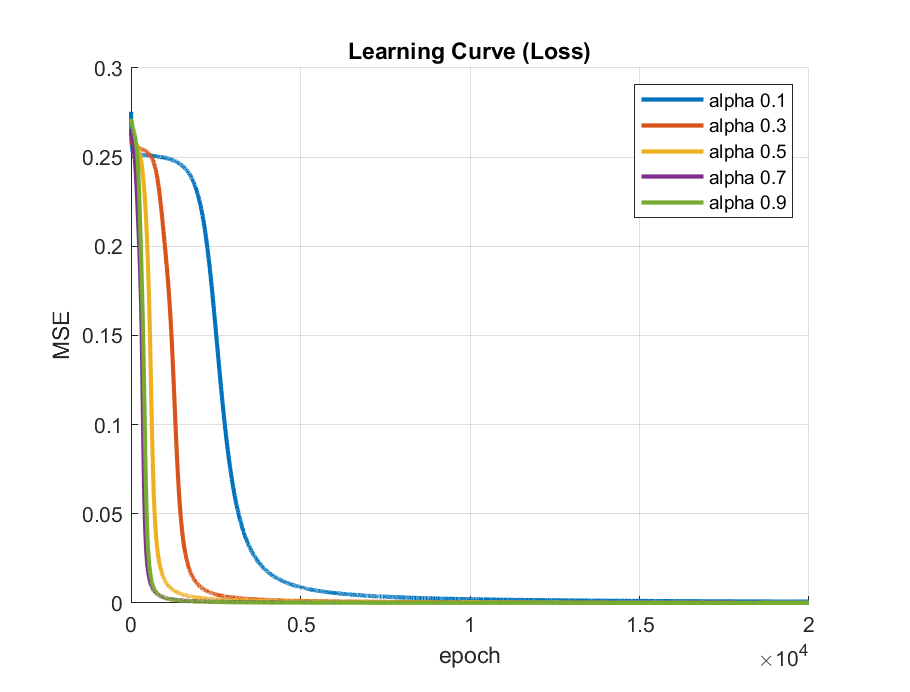
\includegraphics[width=.9\textwidth]{fig6-4nodi-4.eps}}

    \medskip

    \tcbox[boxrule=.3mm,colback=white]{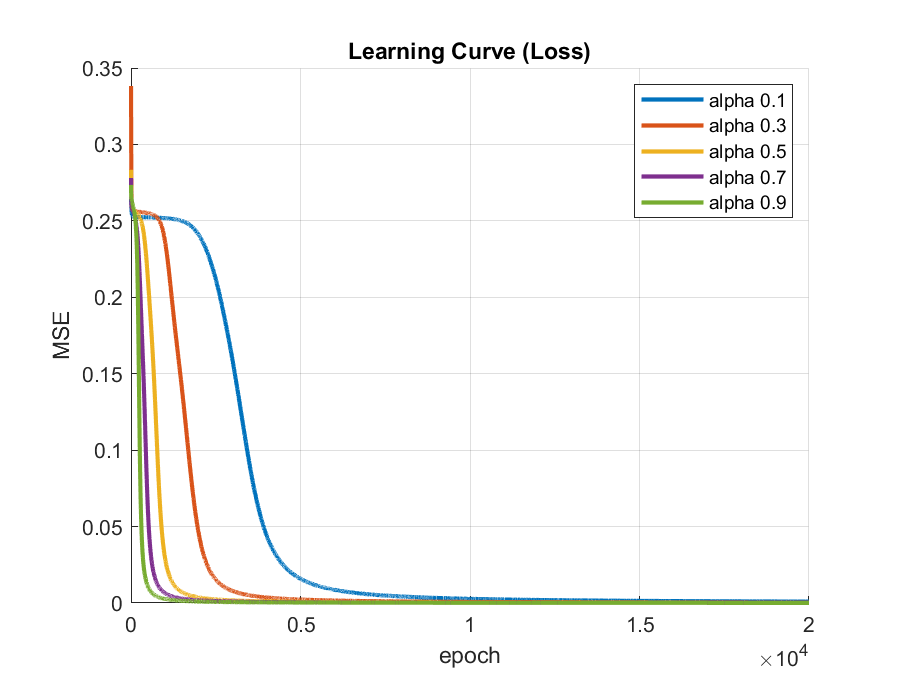
\includegraphics[width=.9\textwidth]{fig6-4nodi-5.eps}}

    \caption{Curve di apprendimento loss (4/5 e 5/5): seconda implementazione, 4 nodi nello strato nascosto.}
    \label{fig6-6}
\end{figure}



\newpage
Ciò che si vede è che, utilizzando 1 o 2 nodi in più c'è sempre convergenza in 20000 epoche, a differenza del modello ``originale'' con due soli nodi nello strato nascosto. In particolare, mentre con tre nodi nello strato nascosto (Figg.~\vref{fig6},~\vref{fig6-2} e~\vref{fig6-3}) si osservano ancora alcune instabilità, soprattutto entro le prime 10000 epoche, con 4 nodi nello strato nascosto (Figg.~\vref{fig6-4},~\vref{fig6-5} e~\vref{fig6-6}) la convergenza è sempre rapida e garantita, ad eccezione del secondo grafico in cui una curva converge in più tempo (circa 15000 epoche).


\end{document}